\section{New Beam Screen Designs}

Using the knowledge acquired from examining the beam coupling impedance dependence on the layout of the beam screen from the previous section, and additionally the electrical field simulations of the induced voltages on the screen conductors during magnet firing and number of alternative beam screen designs have been proposed. The driving points in these designs has been to reduce the power loss into the MKI (in this case to reduce the temperatures reached by the ferrite yoke) and to reduce the induced voltage in the screen conductors during magnet firing to eliminate electrical breakdown/discharge between the screen conductors and along the end the surface of the beam screen to a ground plane.

The proposed designs are described below:

\begin{itemize}
\item{24 screen conductors of alternating length, as shown in Fig.~\ref{fig:24-alternating-length}. The alternating length screen conductors layout has been demonstrated to reduce the induced voltage on the shorter length screen conductors, thus being beneficial to the electrical breakdown rate.}
\item{24 screen conductors tapered in length, as shown in Fig.~\ref{fig:24-tapered-length}. The tapering of the screen conductors has previously been shown to help reduce the induced potential in designs with 15 screen conductors, and should be kept as a proven, if not optimal option for 24 screen conductors.}
\item{24 screen conductors some with an alternating length and then tapered towards the HV busbar, as shown in Fig.~\ref{fig:24-alternating-tapered}. This intended to use the reduction of induced voltage due to the tapering, whilst keeping a relatively high capacitance at the capacitively coupled end so as to not induce additional worse resonances here.}
\item{24 screen conductors in enclosed slots in the ceramic beam screen, as shown in Fig.~\ref{fig:24-enclosed-slots}. The intention of this design is to increase the necessary induced voltage on the screen conductors before breakdown occurs due to surface tracking no longer being a possible breakdown path.}
\item{An alternative screen conductor layout, in which some are conductively connected to ground on both ends and all other capacitively coupled, as shown in Fig.~\ref{fig:alt-screen-design}. This design is intended to reduce the induced voltage on the screen conductors by having all the screen conductors be connected to one another at the capacitively coupled end thus receiving the same induced voltage. To counter possible eddy currents during firing reducing the field rise time the majority of the screen conductors are capacitively coupled at both ends of the magnet, with two conductors conencted to ground at the downstream end of the magnet.}
\item{24 screen conductors with part of the metallization replaced by a external metal cylinder, as shown in Fig.~\ref{fig:24-step-out-slight}. This design is intended to reduce the electric field gradients at the capacitively coupled end by removing the distance between the screen conductors and the ground plane by replacing the metallization on the external surface of the ceramic beam screen with a metal cylinder some millimetres off the surface. Electric field simulations had shown that the high permittivity of the ceramic was in effect pushing the ground plane into the ceramic cylinder, reducing the effective spacing between the screen conductors and the metallization, whereas this physical air gap should reduce this effect.}
\item{24 screen conductors of a mixture of alternating and tapered lengths with part of the metallization replaced with an external metal cylinder, as shown in Fig.~\ref{fig:24-final-design}. This was intended to improve on the above design by using the combined alternating and tapered design to further reduce the induced voltages on the screen conductors. Due to difficulty of manufacturing the step out of the beam screen is continued beyond the ends of the screen conductors. \textbf{This is the proposed final design for implementation in the replacement MKIs for installation during long shutdown 1}.}
\end{itemize}

\begin{figure}
\begin{center}
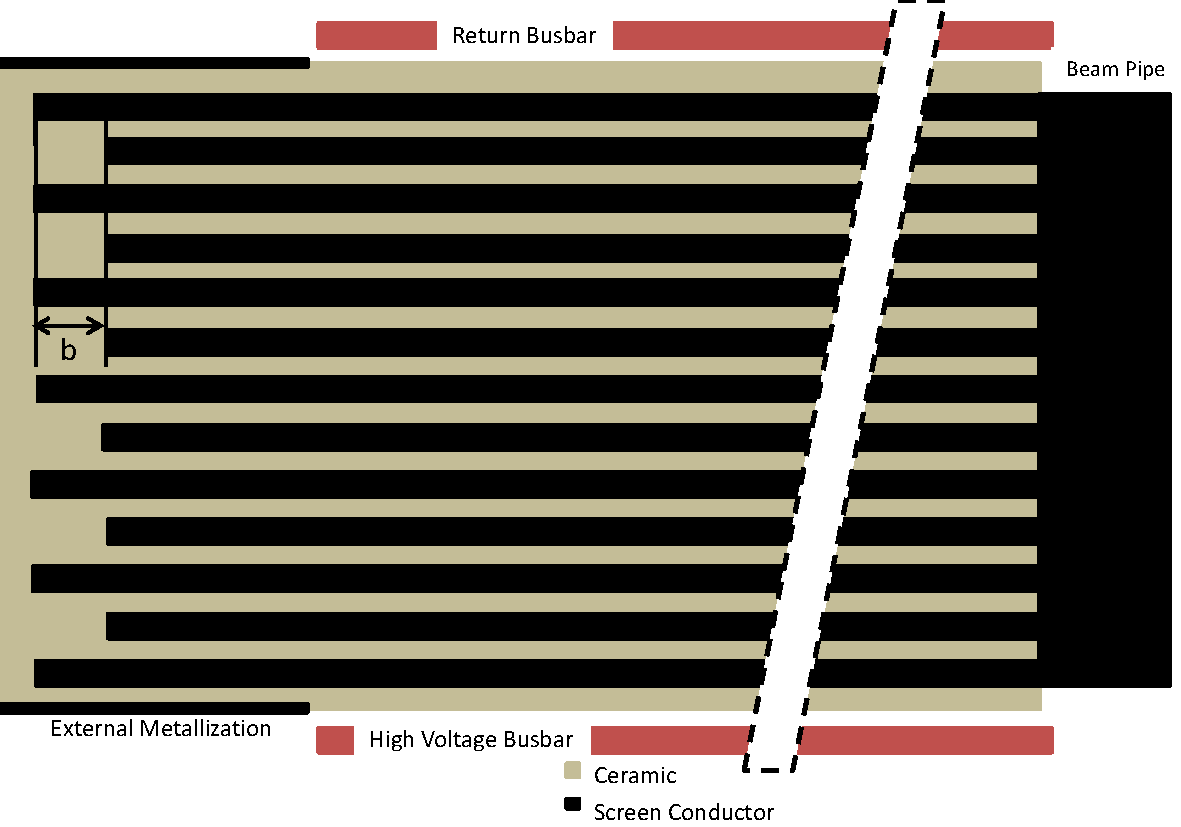
\includegraphics[width=0.7\textwidth]{LHC_MKI/figures/mki-design-layouts/alternating_screen_conductors.pdf}
\end{center}
\label{fig:24-alternating-length}
\caption{A MKI beam screen design with alternating lengths of screen conductors - seperated by a length b.}

\end{figure}
\begin{figure}
\begin{center}
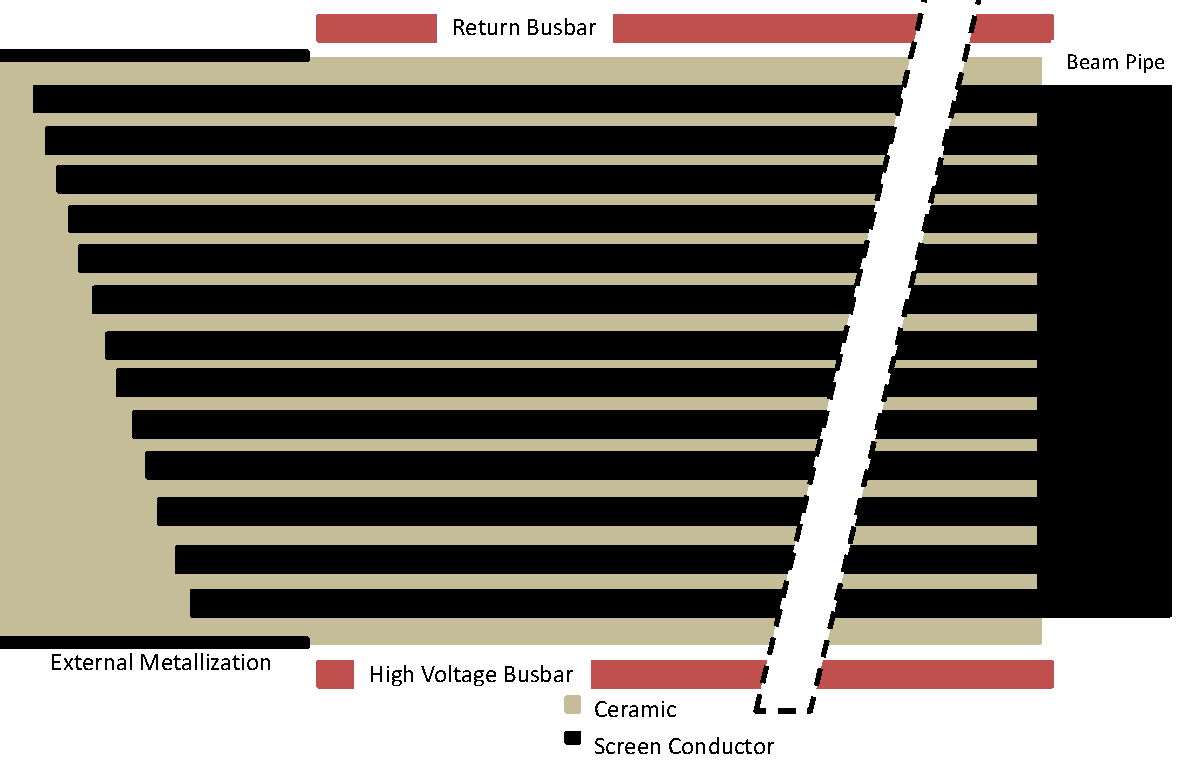
\includegraphics[width=0.7\textwidth]{LHC_MKI/figures/mki-design-layouts/shortening_screen_conductors.pdf}
\end{center}
\label{fig:24-tapered-length}
\caption{A MKI beam screen design with tapered lengths of screen conductors. The taper may be altered to acquire the desired combination of impedance and induced voltage on the screen conductors.}
\end{figure}
\begin{figure}
\begin{center}
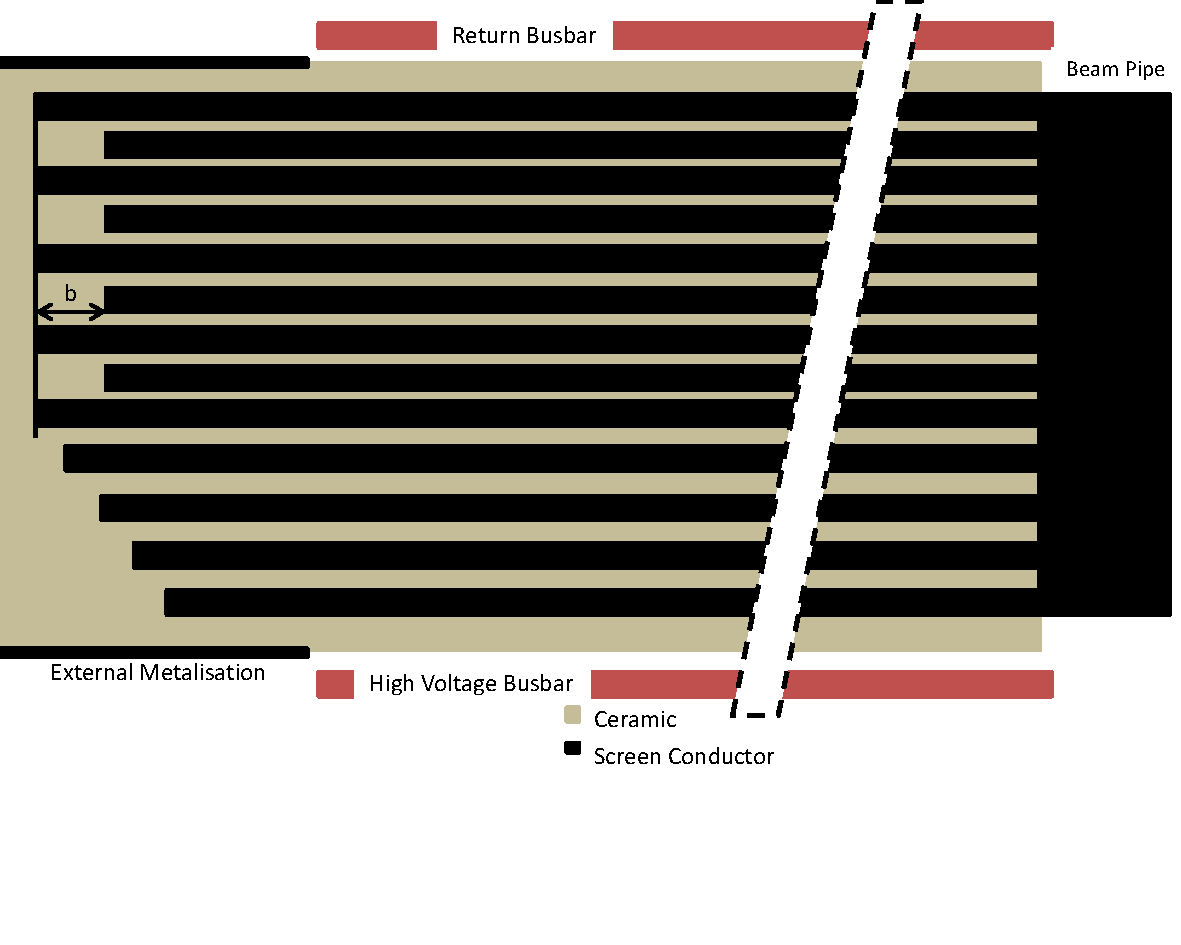
\includegraphics[width=0.7\textwidth]{LHC_MKI/figures/mki-design-layouts/combination_layout.pdf}
\end{center}
\label{fig:24-alternating-tapered}
\caption{A MKI beam screen design with a combination of tapered and alternating screen conductors. The degree of alternating and tapering may change dependent of the desired impedance and induced voltage on the screen conductors.}
\end{figure}

\begin{figure}
\begin{center}
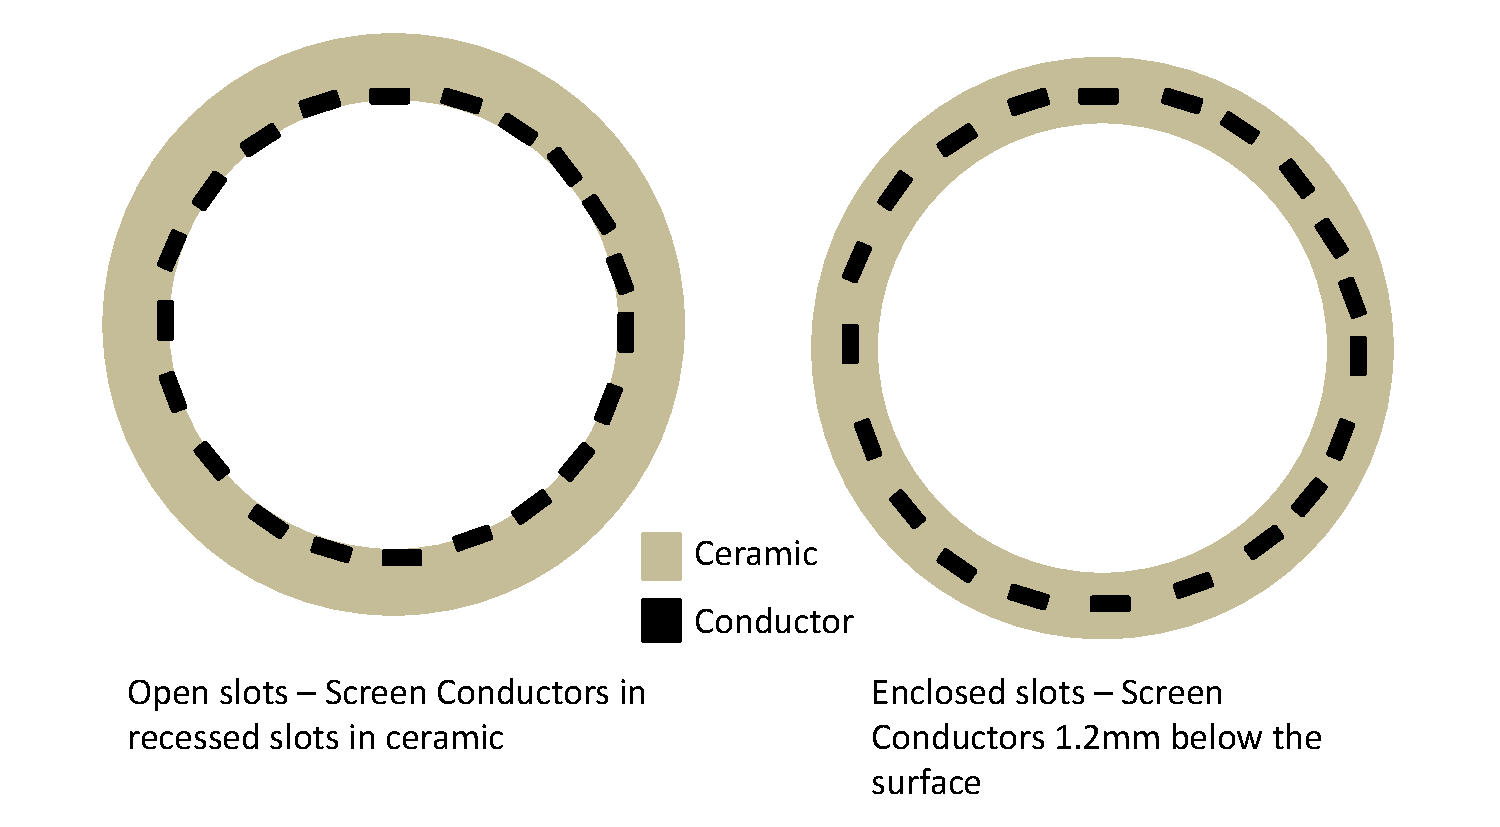
\includegraphics[width=0.7\textwidth]{LHC_MKI/figures/mki-design-layouts/enclosed_diagram.pdf}
\end{center}
\label{fig:24-enclosed-slots}
\caption{A MKI beam screen design with enclosed slots (shown in comparison to the usual beam screen design with open slots) for the screen conductors.}
\end{figure}

\begin{figure}
\begin{center}
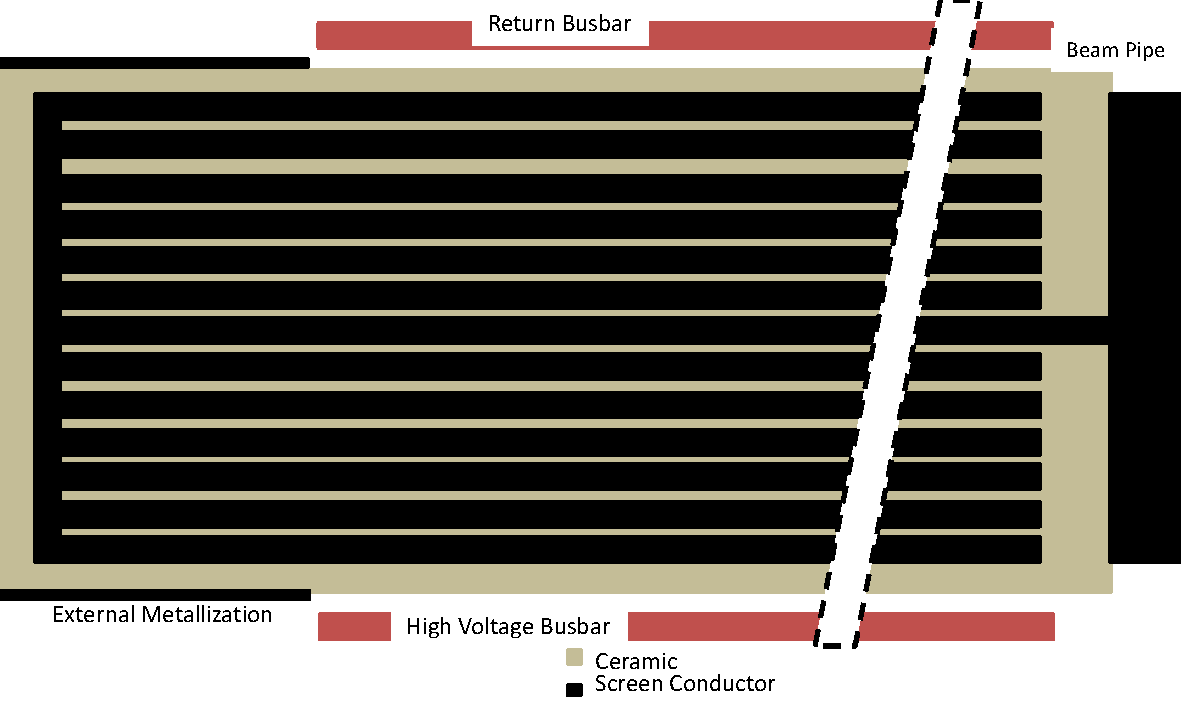
\includegraphics[width=0.7\textwidth]{LHC_MKI/figures/mki-design-layouts/alternative_screen_design.pdf}
\end{center}
\label{fig:alt-screen-design}
\caption{A MKI beam screen design using an alternative screen conductor layout in which 2 (cross section shown here) conductors are connected to ground at the downstream end of the screen, and all conductors are welded together are the capacitiviely coupled end.}
\end{figure}

\begin{figure}
\begin{center}
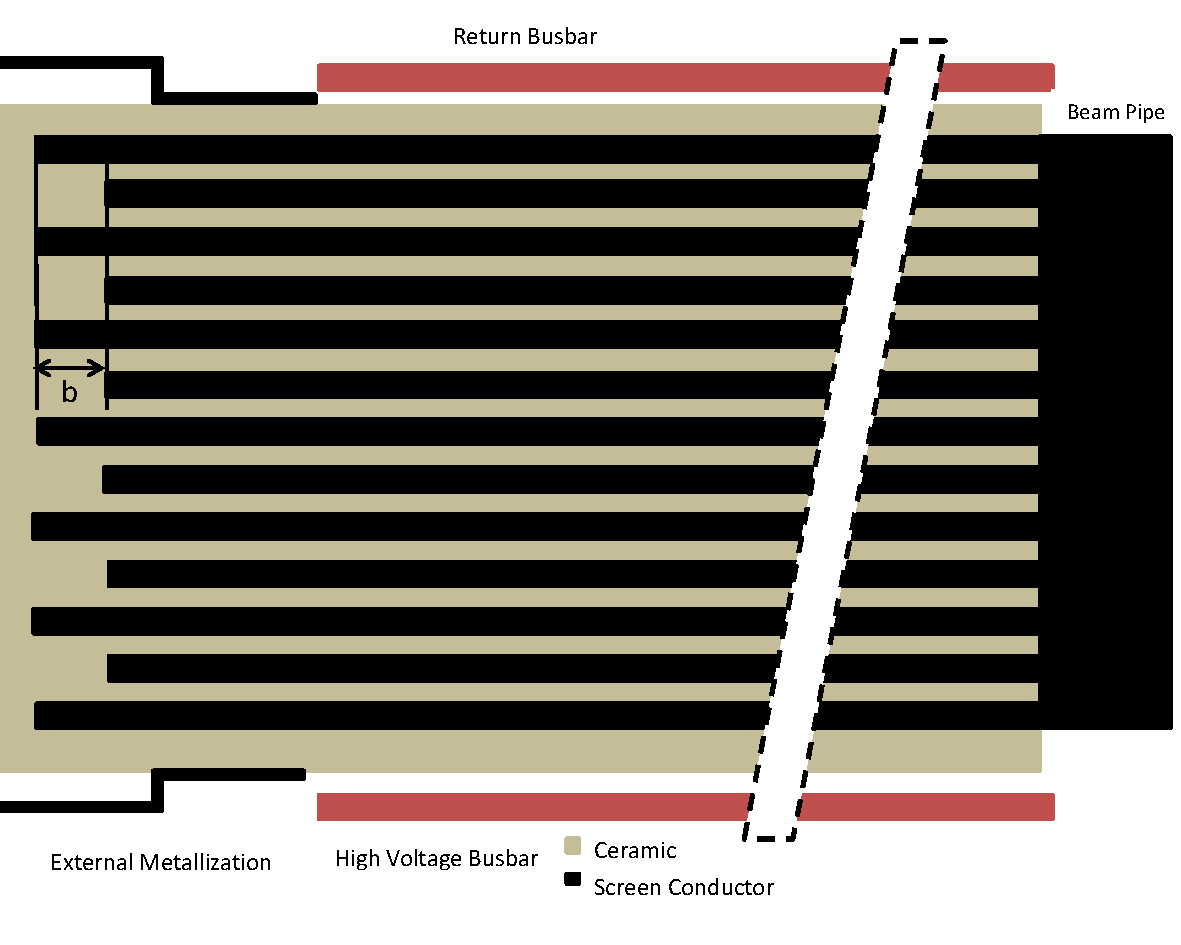
\includegraphics[width=0.7\textwidth]{LHC_MKI/figures/mki-design-layouts/alternating_screen_conductors_step_out_metallisation.pdf}
\end{center}
\label{fig:24-step-out-slight}
\caption{A MKI beam screen design implementing a replacement of some of the external metallization with a metallic cylinder so as to pull the ground plane closest to the screen conductors away.}
\end{figure}

\begin{figure}
\begin{center}
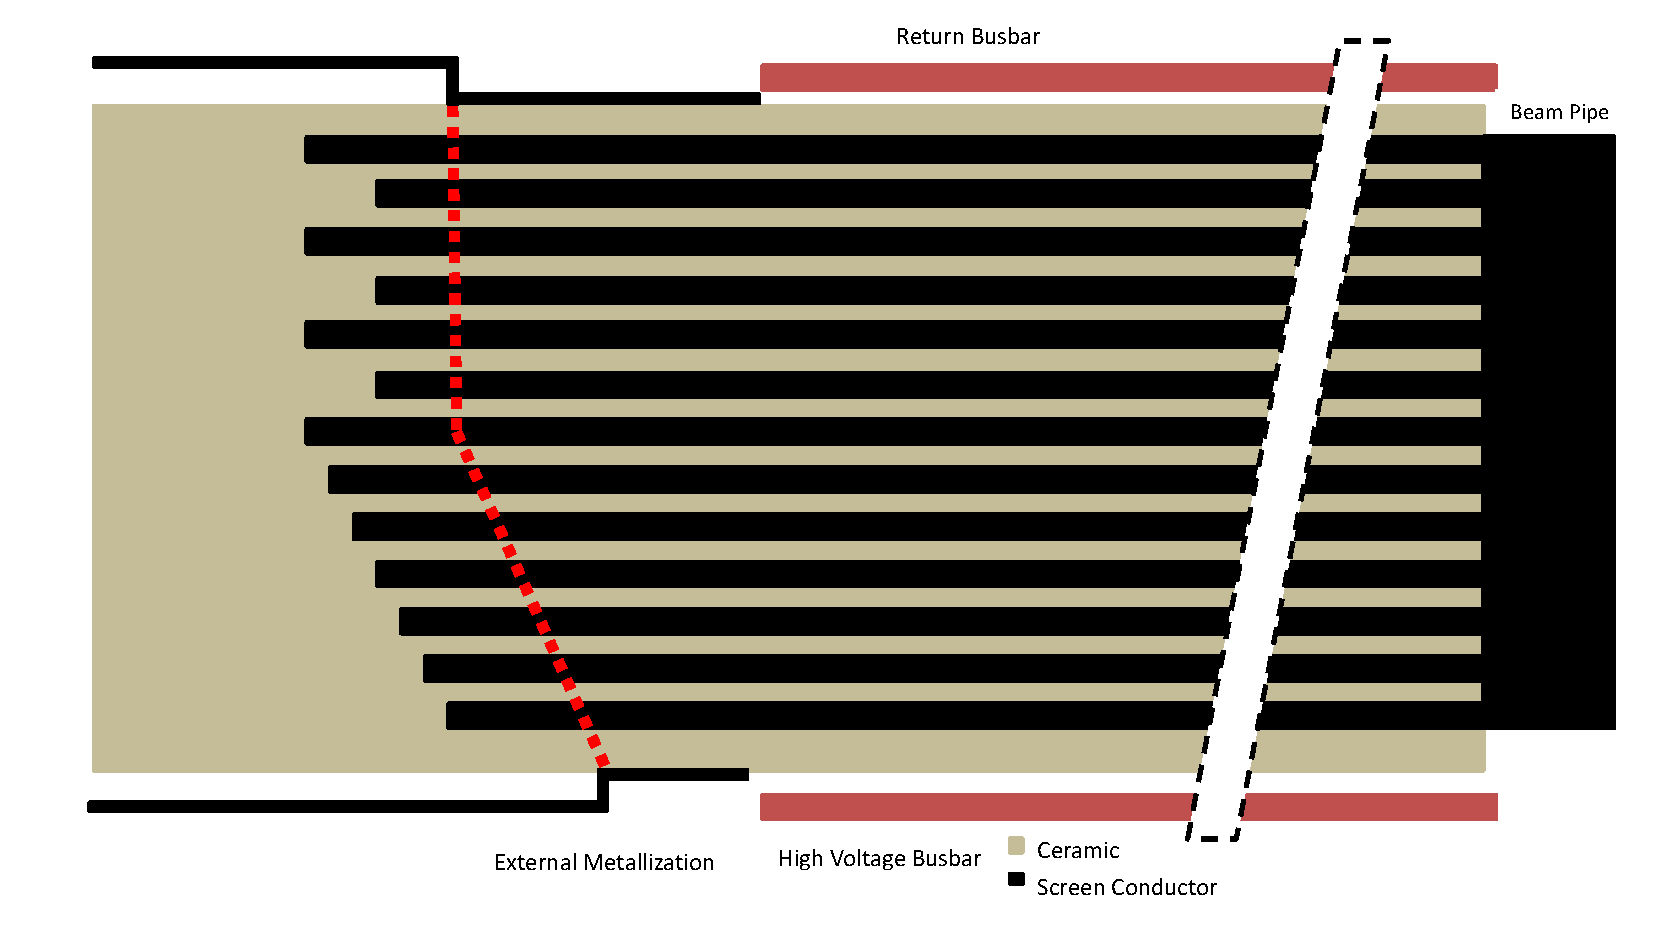
\includegraphics[width=0.7\textwidth]{LHC_MKI/figures/mki-design-layouts/mki-final-design.pdf}
\end{center}
\label{fig:24-final-design}
\caption{The proposed final MKI design. A combination of alternating and tapered screeb conductors is used, along with a step out of the external metallization. The outline of the step out is shown by the red-dashed line.}
\end{figure}

In this analysis we shall focus on the resulting power loss from interaction of the beam with the real component of the longitudinal beam impedance as this is the present primary limitation from the MKIs. The real component of the longitudinal beam coupling impedance is shown in Fig.~\ref{fig:new-screen-designs-mki} along with comparisons to the existing MKIs in the LHC with 15 and 19 screen conductors. A restricted selection of the results (combination layout from Fig.~\ref{fig:24-alternating-tapered}, the alternative design from Fig.~\ref{fig:alt-screen-design} and the final design Fig.~\ref{fig:24-final-design}) logarithmic (i the y-axis) plot is shown in Fig.~\ref{fig:new-screen-designs-mki-log} for further clarity.

\begin{figure}
\begin{center}
\subfigure[]{
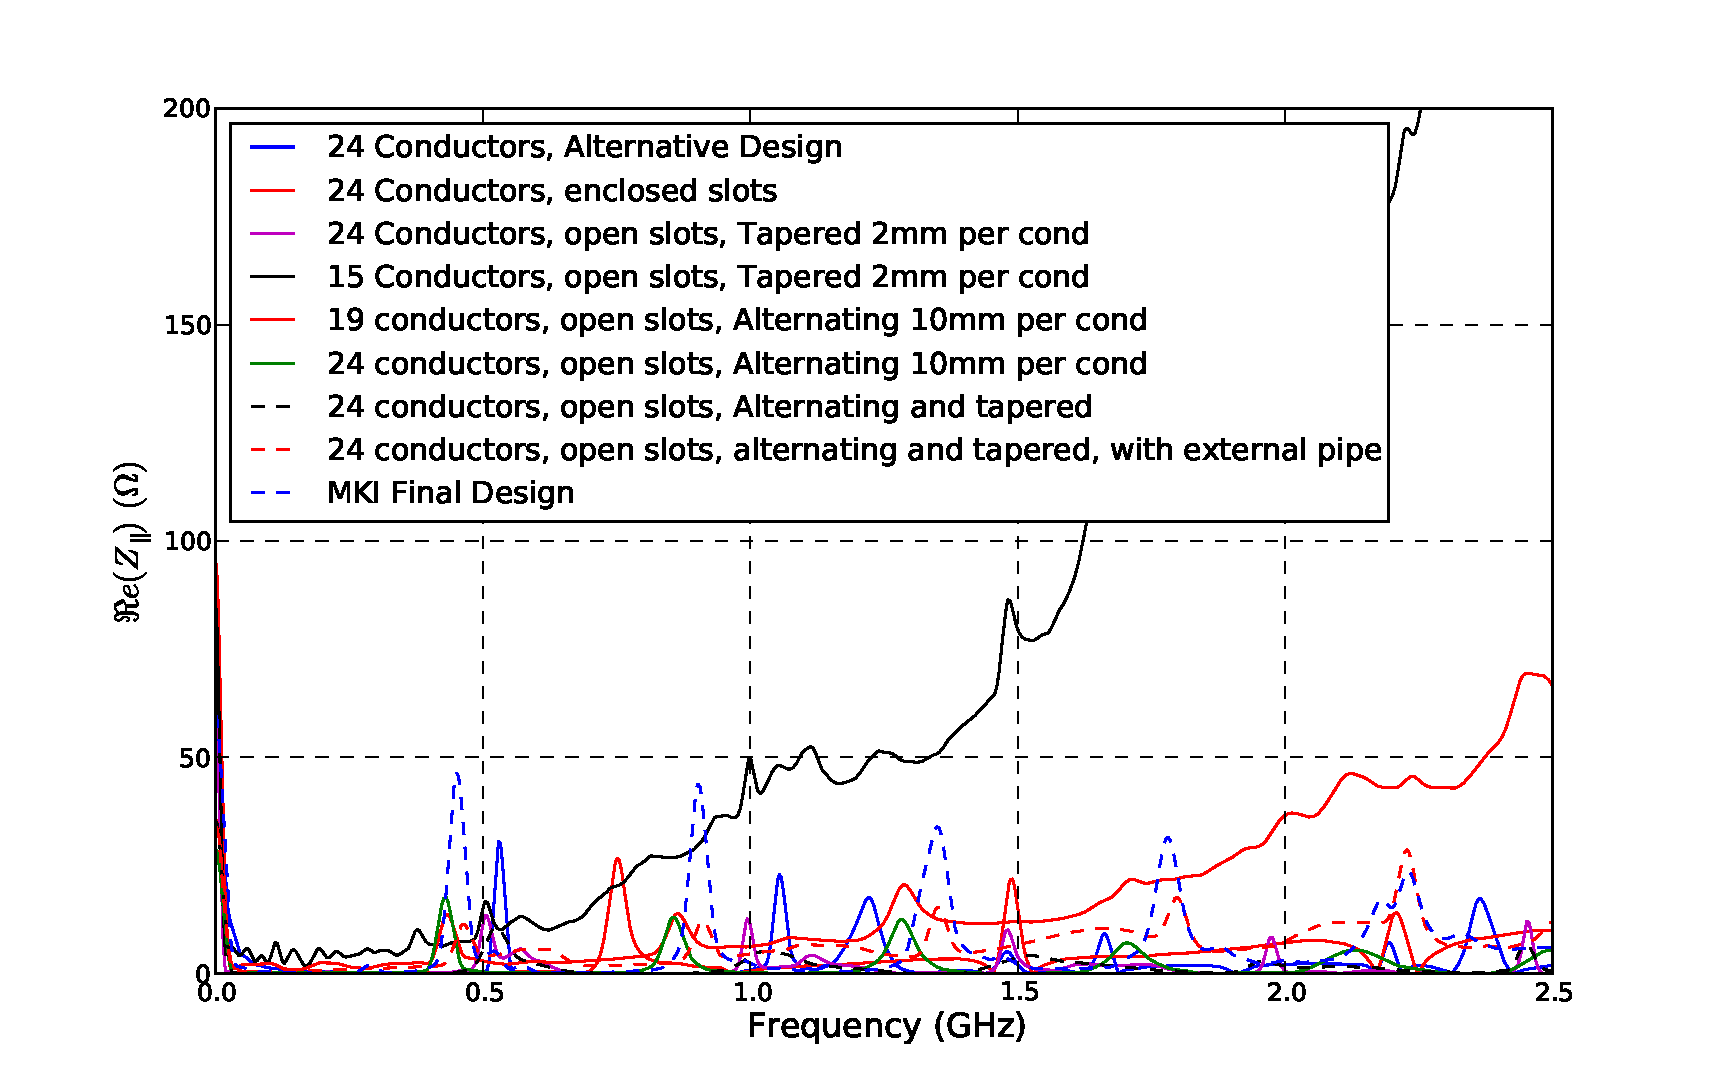
\includegraphics[width=0.75\textwidth]{LHC_MKI/figures/mki-new-screen-designs-impedance.pdf}
\label{fig:new-screen-designs-mki}
}
\subfigure[]{
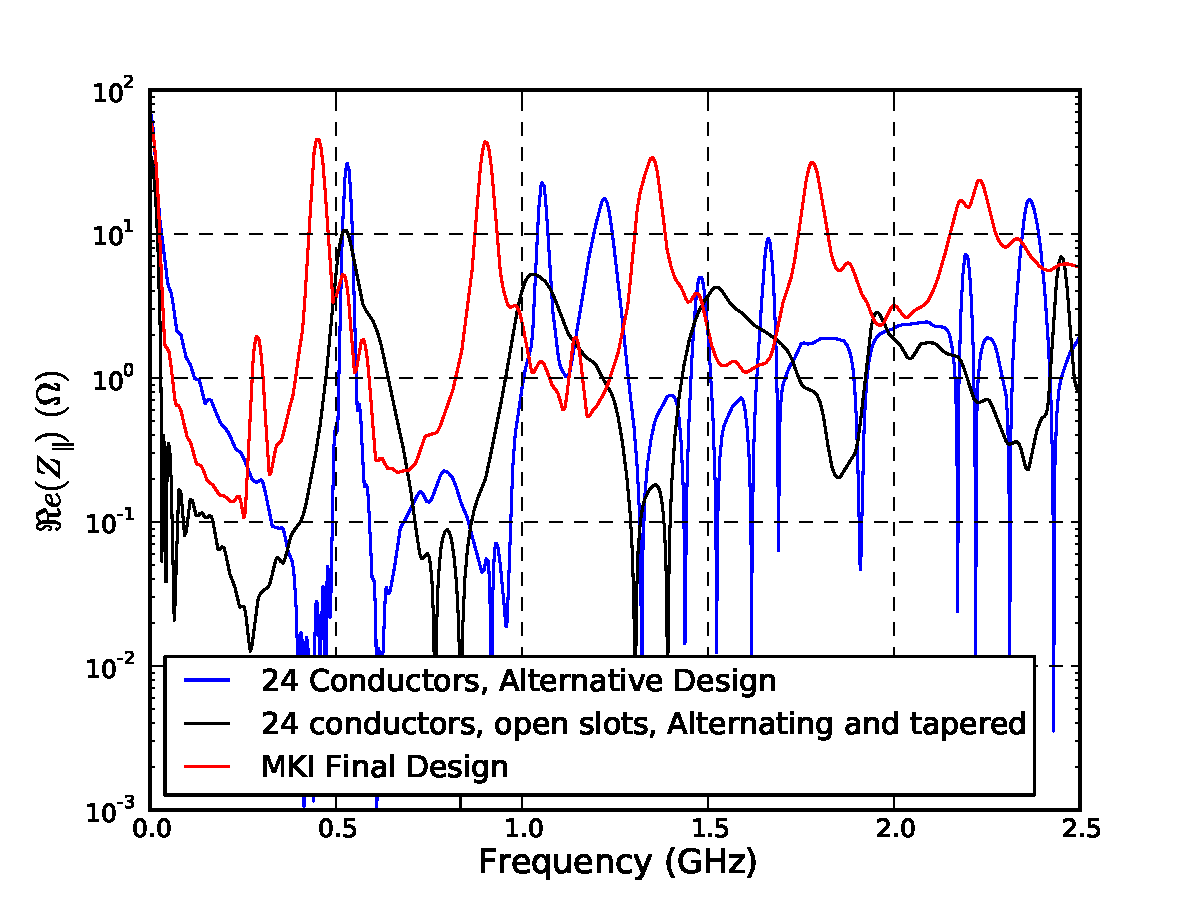
\includegraphics[width=0.75\textwidth]{LHC_MKI/figures/mki-new-screen-designs-impedance-log.pdf}
\label{fig:new-screen-designs-mki-log}
}
\end{center}
\caption{The real component of the beam coupling impedance for a number of the proposed beam screen designs compared to the existing designs (15 screen conductors tapered and 19 screen conductors alternating in length) \ref{fig:new-screen-designs-mki}. A selected collection of favourable (from the impedance and the electric field point of view) are shown in \ref{fig:new-screen-designs-mki-log} with a log scale on the Y axis so the resonance structure can be more clearly seen.}
\end{figure}

The estimated heating for both 25ns and 50ns bunch spacing operation in the LHC are shown in Tab.~\ref{tab:heating-mki-screen-designs} for 1ns bunch length, and the variation in power loss with the bunch length for 25ns and 50ns bunch spacing shown in Fig.~\ref{fig:mki-screens-heating-bunch-length}. It can be seen that the power loss can be very strongly reduced for very short bunch lengths (as has been proposed for HL-LHC operation without crab cavities [cite]) by increasing the bunch length, but for nominal bunch lengths ($\tau_{b}=$1ns) it can be seen that there is not much benefit in increasing the bunch length.

\begin{table}
\label{tab:heating-mki-screen-designs}
\caption{The power loss expected due to beam-wakefield interactions in the MKIs for a number of proposed beam screen designs. Estimates are given for 50ns and 25ns bunch spacing in the LHC (1380 bunches, $1.7 \times 10^{11}$ particles per bunch for 50ns, 2808 bunches, $1.15 \times 10^{11}$ particles per bunch for 25ns) assuming a cos$^{2}$ bunch distribution.}
\begin{center}
\begin{tabular}{c | c | c}
Screen Design & $P_{loss,50ns}$ (W), $t_{b}=1$ns & $P_{loss,25ns}$ (W), $t_{b}=1$ns \\ \hline 
24 Conductors, Alternating Length & 36 & 28 \\ \hline %full length
24 Conductors, Tapered Length & $P_{loss,50ns}$ (W), $t_{b}=1$ns & $P_{loss,25ns}$ (W), $t_{b}=1$ns \\ \hline %full length
24 Conductors, Alternating and Tapered & $P_{loss,50ns}$ (W), $t_{b}=1$ns & $P_{loss,25ns}$ (W), $t_{b}=1$ns \\ \hline %full length
24 Screen Conductors, Enclosed Conductors & $P_{loss,50ns}$ (W), $t_{b}=1$ns & $P_{loss,25ns}$ (W), $t_{b}=1$ns \\ \hline %no shortened
24 Conductors, Alternate Design & $P_{loss,50ns}$ (W), $t_{b}=1$ns & $P_{loss,25ns}$ (W), $t_{b}=1$ns \\ \hline %no shortened
24 Conductors, Step out & 37 & 28 \\ \hline %Shortened
24 Conductors, Final Design & 37 & 28 \\ %full length
\end{tabular}
\end{center}
\end{table}

\begin{figure}
\subfigure[]{
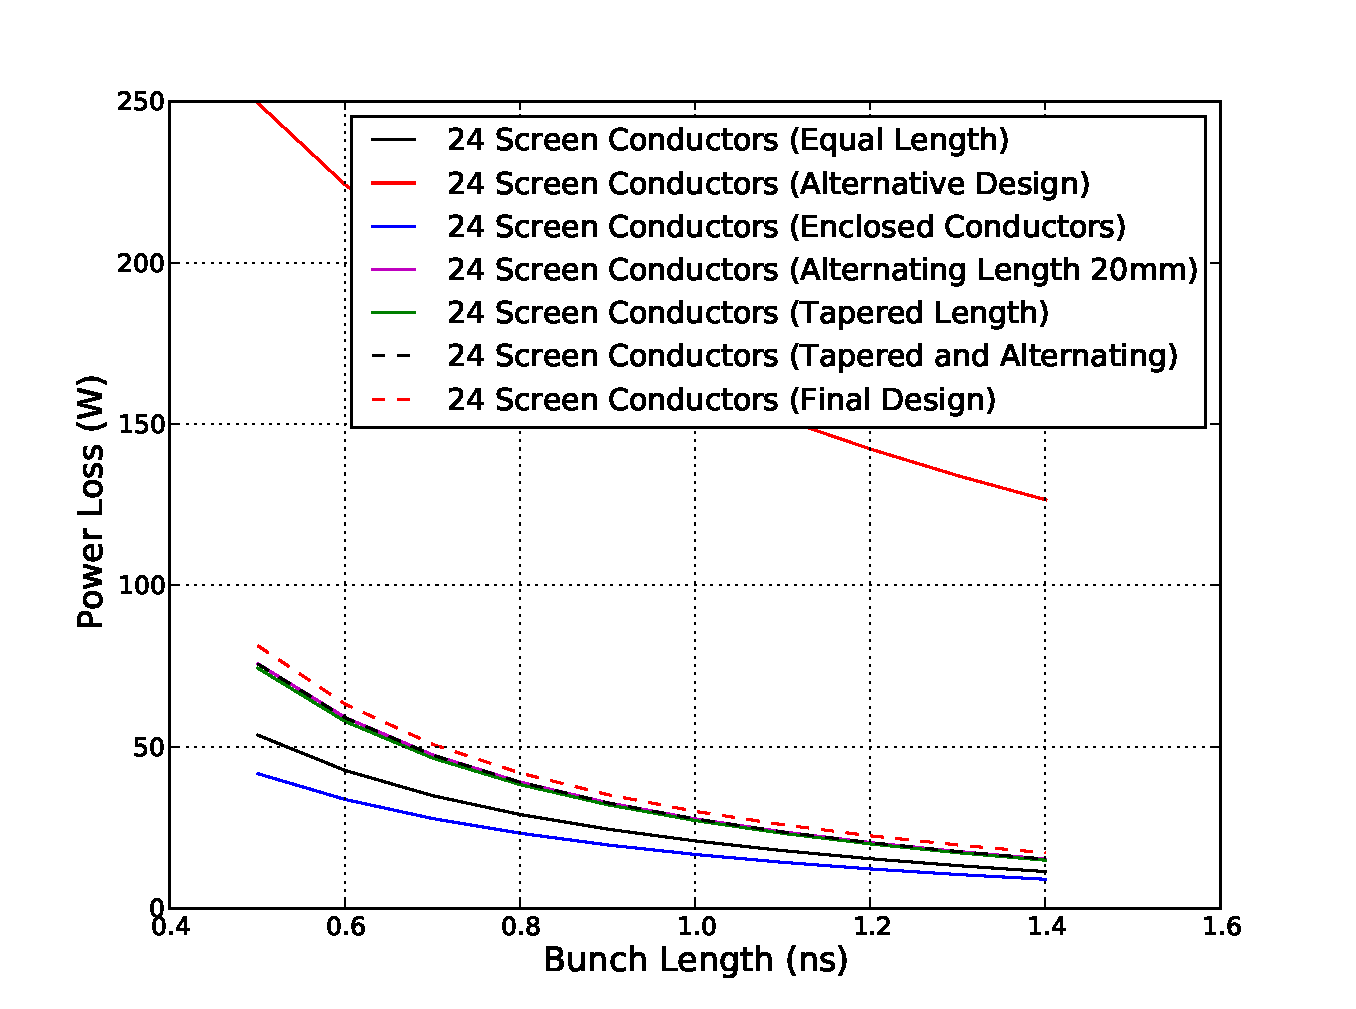
\includegraphics[width=0.5\textwidth]{LHC_MKI/figures/mki-new-designs-heating-25ns.pdf}
\label{fig:mki-screen-heating-25ns}
}
\subfigure[]{
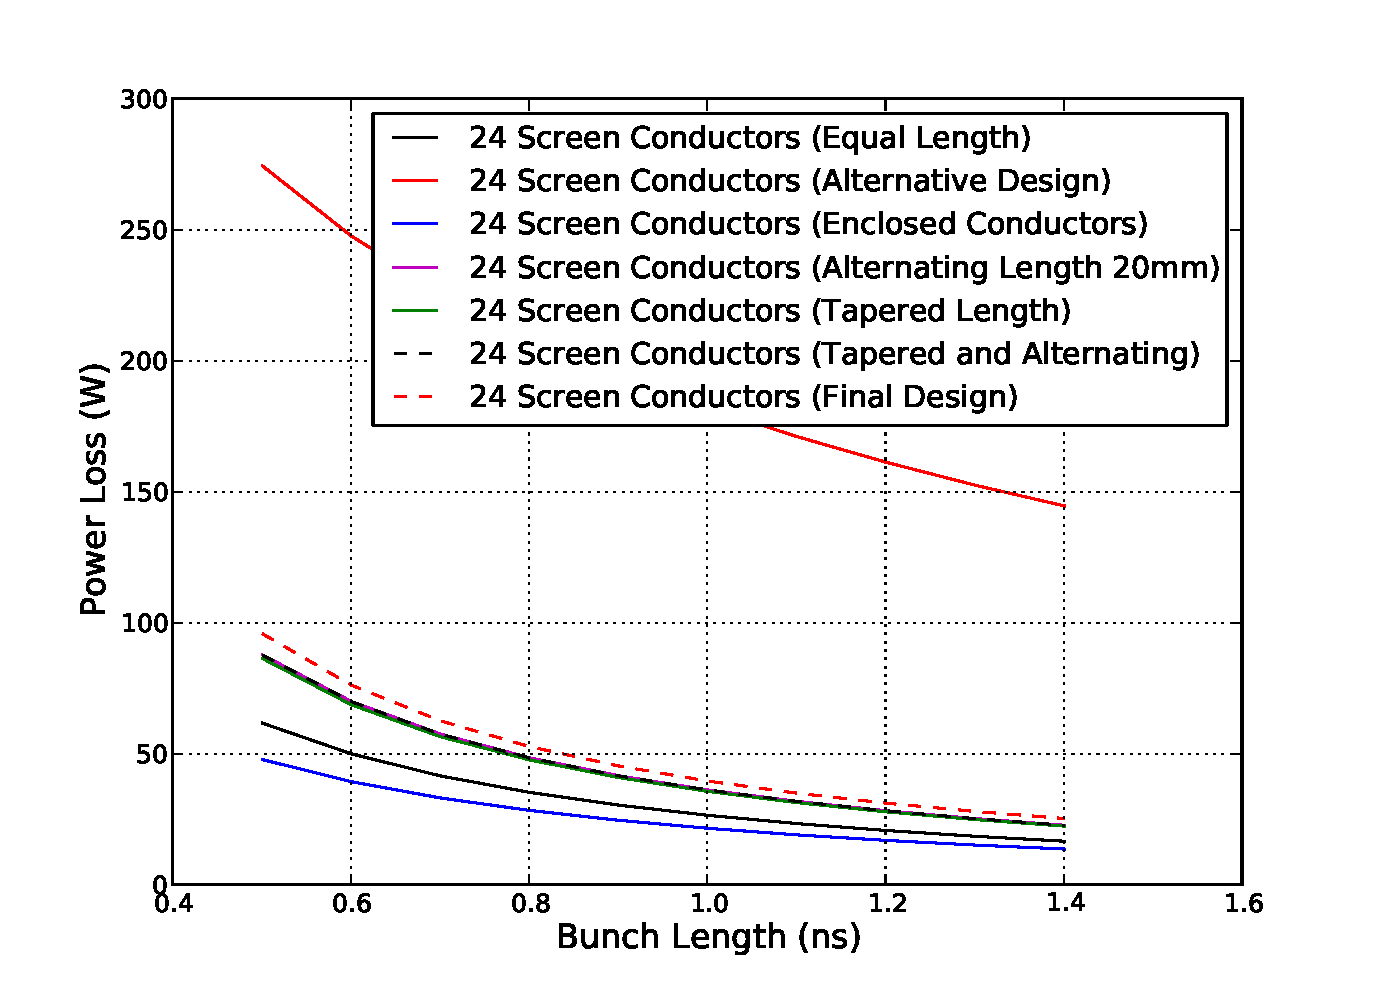
\includegraphics[width=0.5\textwidth]{LHC_MKI/figures/mki-new-designs-heating-50ns.pdf}
\label{fig:mki-screen-heating-50ns}
}
\label{fig:mki-screens-heating-bunch-length}
\caption{The variation of the predicted beam induced power loss with bunch length for a number of screen designs. The variation for 25ns \ref{fig:mki-screen-heating-25ns} and 50ns \ref{fig:mki-screen-heating-50ns} machine settings.}
\end{figure}
